\section{Geometrical Optics}

This is the thin lens equation for convex (converging) lenses:
$$
	\frac{1}{f} = \frac{n-1}{R_1} + \frac{n-1}{R_2}
$$
For concave lenses, we have that:
$$
	\frac{1}{f} = \frac{-2}{R}
$$
\paragraph{Example}A gun sight is designed to view a distant object at 9x
magnification. If the overall length, $L$, is 10 cm, suggest values of $f_1$ and
$f_2$ where the cross-hair should be placed.
\begin{figure}[h!]
	\centering
	\includegraphics[width=0.7\textwidth]{GunSight.png}
\end{figure}

We have that:
$$
	\tan \alpha = \frac{y}{f_1} \approx \alpha
$$
$$
	\tan \beta = \frac{y}{f_2} \approx \beta
$$
$$
	f_1 + f_2 = 10\; \mathrm{cm}
$$
Since the image is at infinity, we define an angular magnification:
$$
	M = -\frac{\beta}{\alpha}
$$
We know that:
$$
	\beta = -9\alpha
$$
And as such we can find taht:
$$
	\frac{\alpha}{\beta} = \frac{f_2}{f_1}
$$
and that $f_2 = 1$ cm, $f_1 = 9$ cm.

\subsection{$f$-ratio}
The $f$-ratio is the focal length over the diameter: $f/D$. Telescopes with a
low $f$ ratio, e.g. $f/1$, are faster (they take less time to collect the same
amount of light on the sensor).

\subsection{Effective focal length}
The effective focal length is the focal length of the whole compound lens system
if they were replaced with a single large lens. We always give telescope sizes
in diameters rather than in radii.

\subsection{Refracting and reflecting telescopes}
Even though the discussion this far has been on refracting telescopes, they are
seldom used. This is because refracting telescopes need a very long focal length
to be abberation-free, and large lenses are very difficult to make as well as
support. Reflecting telescopes, however, are more common because it is easier to
design them and they are much `faster'. We must make the mirror in a reflecting
telescope \emph{parabolic} rather than circular to prevent abberation.

\subsection{The plate scale}
We define the plate scale as:
$$
	\frac{\mathrm{d}\theta}{\mathrm{d}s}.
$$
From the small angle approximation:
$$
	s = f \theta
$$
The plate scale gives us the number of arcseconds per milimeter that is observed
on the detector.

\paragraph{Example:} We want a field of view of 1'x1'. We have an 8m telescope
with a detector of 128x128 px, with each pixel being 100 $\mu$m across.

\begin{enumerate}
	\item What is the plate scale in arcseconds/mm?
	\item What should the focal length be to achieve this plate scale?
\end{enumerate}

\begin{enumerate}
	\item The physical size of the detector: 
	$$
		128 \times 100 = 12.8 \; \mathrm{mm}.
	$$
	As such we have the plate scale:
	$$
		\frac{\mathrm{d}\theta}{\mathrm{d}s} = \frac{60}{12.8} = 4.7 \;
		\frac{"}{\mathrm{mm}}.
	$$
	\item From above:
	$$
		\frac{\mathrm{d}\theta}{\mathrm{d}s} = \frac{1}{f} \; rightarrow \;
		f = 43.9 \; \mathrm{m}.
	$$
\end{enumerate}
\subsection{Limitations}
We are not really limited by the number of pixels that we can have on a
detector, we can have pretty much as many as we want now. However, we are
limited by the defraction limit of the telescope. When we take an image of a
point source through a circular apeture, we get an airy disk:
\begin{figure}[h!]
	\centering
	\includegraphics[width=0.5\textwidth]{AiryDisk.png}
\end{figure}
With small telescopes, it is hard to resolve individual points that are close
together because the airy disks overlap.
\paragraph{Rayleigh's Criterion} sates that we can resolve two objects if the
primary maximum of one overlaps with the first maximum of the other.

For circular apetures, the angular resolution is:
$$
	\theta_{dl} = \frac{1.22 \lambda}{D}
$$


